\documentclass[a4paper]{article}
%review 


%#########################################################################
\usepackage[utf8]{inputenc}
%\usepackage[T1]{fontenc}
%\usepackage[francais]{babel}
%\usepackage{lmodern}
\usepackage[hmargin=4cm, vmargin=2cm, includeheadfoot]{geometry}
\usepackage{alltt}
\usepackage{multicol}
\usepackage{amsmath,amssymb}
\usepackage{color}
\usepackage{graphicx}
\usepackage[francais,bloc,completemulti]{automultiplechoice}     % Mandatory for conversion
\usepackage{mhchem} % needed for chemical equations
\usepackage{tikz}

% exemple de commande utilisateur
\providecommand{\abs}[1]{\lvert#1\rvert}
%#########################################################################
% Entête
%#########################################################################



\title{Test de conversion AMC vers moodle}
\author{BN}



%#########################################################################
% Document
%#########################################################################
\begin{document}

%
% B A R E M E 
% e=incohérence; b=bonne; m=mauvaise; p planché (on ne descent pas en dessous)
\baremeDefautS{e=-0.5,b=1,m=-0.5}% never put b<1,
\baremeDefautM{e=-0.5,b=1,m=-0.25,p=-0.5}% never put b<1, with amc2moodle m correspond to the grade if all the wrong answers are ticked, b correspond to the grade if all the good answers are ticked




%question : environnement, text question
%element{label}{groupe} :commande, encapsule la commande pour lui donner un groupe
%reponses : environnement
%bonne  : commande
%mauvaise : commande
% B A R E M E 
% e=incohérence; b=bonne; m=mauvaise; p planché (on ne descent pas en dessous)
%\baremeDefautS{e=-0.5,b=1,m=-0.5}
%\baremeDefautM{e=-0.5,b=0.5,m=-0.25,p=-0.5}
% ajouter aucune de ces réponses n'est correcte
%\usepackage[francais,bloc,completemulti]{automultiplechoice}  

%===================================================================
% simple
\element{cat1}{
  \begin{question}{Qsimple:img}
    On souhaite faire passer \textit{exactement}, par $N$ points donnés, un \texttt{polynôme} de degré \textbf{strictement} égal à $N-1$. Pour trouver les coefficients on doit résoudre un \emph{problème}
    %\attachfile{./a.c}
    %\includesounds{./Son/piano2.mp3} % test pour inclure sons
    \begin{center}
      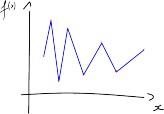
\includegraphics[width=0.5\textwidth]{./Figures/other/schema_interpL.png}
    \end{center}

    \begin{reponses}
      \bonne{d'interpolation}
      \mauvaise{de moindre carré}
      \mauvaise{de Thelonius Sphere Monk
        \begin{flushright}
          
\includegraphics[height=2cm]{./Figures/tinymonk.pdf}
        \end{flushright}
        \begin{flushleft}
          
\includegraphics[height=3cm]{./Figures/tinymonk.pdf}
        \end{flushleft}
      }
    \end{reponses}
  \end{question}
}

%
%===================================================================
% questions à réponse multiple
% pas de bonne réponse, on doit ajouter un champ "aucune de ces réponses n'est correcte"
\element{cat1}{
  \begin{questionmult}{Qmult:Aucune}  \bareme{e=-0.5,b=1,m=-1.,p=-0.5} % never put b<1,
    Quel fruit possède un noyau?
    \begin{reponseshoriz}[o] % keep answers order
      \mauvaise{La pomme}
      \mauvaise{La tomate}
      \mauvaise{le Kiwi}
      %    \mauvaise{En allant à $$ \int_0^2 x \mathrm{d} x $$ la ligne}
    \end{reponseshoriz}
  \end{questionmult}
}
%
% il y a des bonne réponses et un tableau, verbatim, macro
\element{cat2}{
  \begin{questionmult}{Qmult:TabVerbMacro}
    Quels sont les opérations qui donnent un chiffre présent dans le tableau?
    \begin{center}
      \begin{tabular}{ccc}
        \hline
        12                       & 2                                                    & $2^3$ \\
        \multicolumn{2}{c}{Deux} & 
\includegraphics[height=16pt]{4.png}         \\
        \hline
      \end{tabular}
    \end{center}
    \begin{reponses}
      \bonne{ Ou en \texttt{C} using \texttt{alltt} package
        \begin{alltt}
          int s=-2; \\
          for (int i=0;i<4; i++)\{ \\
          s=i*i+s; \\
          \}
        \end{alltt}
        %        \begin{verbatim}%L'environnement verbatim pose en effet des problèmes avec AMC
        %            int s=0
        %            for(int i;i=0; i<4){
        %            	   s++
        %            } 	               
        %        \end{verbatim}
      }
      \bonne{$\abs{-10-2}$ (math inline and newcommand)}
      \mauvaise{la réponse en image 
\includegraphics[height=16pt]{./Figures/other/4r.png}}
      \mauvaise{$6\times 6$}
      \mauvaise{Avec une équation  $$ \int_0^2 x \mathrm{d} x $$ } % works
      \bonne{Avec une équation matricielle
        \begin{equation}
          \mathrm{det} \begin{pmatrix}1 & 2 \\ -1 & 10 \end{pmatrix} = \begin{vmatrix}1 & 2 \\ -1 & 10 \end{vmatrix}
        \end{equation}
      }
      %    \mauvaise{Avec une autre équation utilisant \texttt{aligned} amsmath environnemnt
      %            \begin{equation}\left\{\begin{aligned}\displaystyle t_{0}&amp;\displaystyle=1/\sqrt{3}\\&#10;\displaystyle t_{i+1}&amp;\displaystyle=\frac{\sqrt{t_{i}^{2}+1}-1}{t_{i}}\end{aligned}\right..
      %            \end{equation}
      %    }        
    \end{reponses}
  \end{questionmult}
}


% test with englisg keywords
% example from http://home.gna.org/auto-qcm/auto-multiple-choice.en/latex.shtml#latex.simple
\element{english}{
  \begin{question}{prez}
    Among the following persons, which one has ever been a President of the French Republic?
    \begin{choiceshoriz}
      \correctchoice{René Coty}
      \wrongchoice{Alain Prost}
      \wrongchoice{Marcel Proust}
      \wrongchoice{with an image 
\includegraphics[height=16pt]{./Figures/other/4r.png}}
    \end{choiceshoriz}
  \end{question}
}

\element{english}{
  \begin{questionmult}{pref}     \scoring{e=-0.5,b=1,m=-.25,p=-0.5}
    Among the following cities, which ones are French prefectures?
    \begin{choices}
      \correctchoice{Poitiers}
      \wrongchoice{Sainte-Menehould}
      \correctchoice{Avignon}
    \end{choices}
  \end{questionmult}
}

% test for itemize and enumerate
\element{cat1}{
\begin{question}{itemize-enumerate}
Test for itemize html rendering,
\begin{itemize}
   \item first item
   \item Second item blablabla 
\end{itemize}
test for enumerate html rendering,
\begin{enumerate}
  \item The first item $x^2$ with math
  \item The second \textbf{item } with bold
\end{enumerate}
    \begin{choices}
      \correctchoice{1 bullet list and 1 ordered list\\ Remarks : the tag in item are ignored.}
      \wrongchoice{    \begin{enumerate}
      					\item The first item $x^2$
      					\item The second \textbf{item}
				      \end{enumerate}
    }
    \end{choices}
\end{question}
}


% test for tikz 
\element{tikz}{
  \begin{question}{tikz:Q1}
    Among the following shape, where is the circle

    \begin{choices}
      \correctchoice{
\begin{tikzpicture}
          \draw (2,2) circle (1cm);
        \end{tikzpicture}}
      \wrongchoice{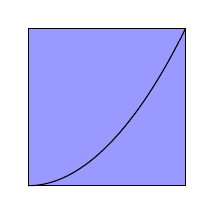
\begin{tikzpicture}
          \filldraw[fill=blue!40!white, draw=black] (0,0) rectangle (2,2);
          \draw (0,0) parabola (2,2);
        \end{tikzpicture}}
      \wrongchoice{$\triangle$}
    \end{choices}
  \end{question}
}

% test for mhchem support with mathjax
\element{mhchem}{
\begin{question}{mathjax-mhchem}
Here is a test for \texttt{mhchem}-\LaTeX package. This package is not yet supported by LaTeXML, thus the rendering is delegated to \texttt{mathjax}. To use it, you need to add \texttt{mhchem} in the \texttt{mathjax} moodle plugin (ask to admin, see details in README file).


A complicated chemical equation \ce{Hg^2+ ->[I-] HgI2 ->[I-] [Hg^{II}I4]^2-}, the same written in math mode : $\ce{Hg^2+ ->[I-] HgI2 ->[I-] [Hg^{II}I4]^2-}$, combine with other math operator $K=\ce{Hg^2+ ->[I-] HgI2 ->[I-] [Hg^{II}I4]^2-}$ and finally placed in the equation environment
\begin{equation*}
K=\ce{Hg^2+ ->[I-] HgI2 ->[I-] [Hg^{II}I4]^2-}
\end{equation*}
% the answers
    \begin{choices}
      \correctchoice{a simpler one \ce{CO2 + C -> 2 CO}.}
      \wrongchoice{Wrong Choice! }
    \end{choices}
\end{question}
}

% test for numerical question support
\element{num}{
\begin{questionmultx}{with-int}
Combien de fois le programme suivant affiche-t-il \texttt{"x"} ?

\texttt{for (int i = 4; i < 24; ++i)\\
\hspace*{1em}for (int j = i + 2; j - 1 > 0; -{}-j)\\
\hspace*{2em}puts("x");}

\AMCnumericChoices{290}{digits=3,sign=false,scoreexact=2,scoreapprox=1,approx=10}
\end{questionmultx}}

% -----------------------------------------------------------------------------
\element{open}{
  \begin{question}{Essai}\label{q:Essai}   
    Explain in few words the aim of this course.
% It is possible to add more granularity with partially correct answer using \wrongchoice[P]{p}\scoring{0.5}
\AMCOpen{lines=2}{    \correctchoice[OK]{OK}    \wrongchoice[F]{F}}
  \end{question}
}


% #################################################################
% C R E A T I O N  D E S  C O P I E S
% #################################################################
\exemplaire{1}{    	% nombre de sujet différent

  %debut de l'en-tête des copies :    

  \vspace*{.5cm}
  \begin{minipage}{.4\linewidth}
    \centering\large\bf Test
  \end{minipage}
  \champnom{\fbox{
      \begin{minipage}{.5\linewidth}
        Nom et prénom :

        \vspace*{.5cm}\dotfill
        \vspace*{1mm}
      \end{minipage}
    }}

  \begin{flushleft}
    Certaine question peuvent sembler étrange, c'est le but !
    \begin{center}
      \Large{\textsc{QCM using AMC Latex Format}}\\
      \normalsize
    \end{center}
  \end{flushleft}



  % mélange et catégorie (groupe dans ACM)
  \cleargroup{BigGroupe}
  \copygroup{cat1}{BigGroupe}
  \copygroup{cat2}{BigGroupe}
  \copygroup{english}{BigGroupe}
  \copygroup{tikz}{BigGroupe}
  \copygroup{mhchem}{BigGroupe}
  \copygroup{num}{BigGroupe}
  \copygroup{open}{BigGroupe}
  % not usefull for testing !
  %\melangegroupe{BigGroupe}
  \restituegroupe{BigGroupe}
}




\end{document}
